\chapter{Utilizing the Framework: Data Market Places}
\label{ch:cmf}

Until this point, this thesis has introduces tools and methodologies for modelling and designing norm-governed (multi-agent) systems. This chapter utilizes those tools to illustrate, implement and analyze a model of a Data Market-Place as a normative multi-agent system. Norms in this context are used as a fully distributed coordination and monitoring mechanism between participants of the market. The goal of the chapter is two-fold: (1) illustrate how such models can be valuable assets for system designers and policy makers by providing insights and generating design artifacts, and (2) as part of the DL4LD project, propose a flexible yet powerful schema and method for development of a data market place.

\section{Introduction}
The intrinsic and potential value of data in many different aspects of human society can not be overestimated, from financial \cite{Hasan2020} to scientific research \cite{Yuri2013} and healthcare \cite{Shilo2020}, every important sector is impacted, and arguably improved in their effectiveness\footnote{At least subjectively improved.} by utilizing data-oriented approaches. Intuitively, the importance of data-sharing between parties is also rising, which in turns creates concern about data security, privacy, legal, monopoly and many other issues specially in the contexts that parties may not have full trust towards each other or are even competitors \cite{clifton2004privacy} creating the need for governance approaches that go beyond single organization scenarios. 

The idea of Data Market Places (DMPs) is one that addresses these issues, a DMP is a membership organization that each member can only perform actions such as transferring data and execution of algorithms based on previously constructed contractual agreements \cite{Zhang2019ModelingPlaces,Shakeri2019}, consortium policies and legislative regulations (e.g., GDPR) for specific purposes. Intuitively, such framework can induce collaboration and add much needed trust between parties knowing their artifacts (data, algorithm, processing power, infrastructure, etc.) are only utilized in the intended manner.

Although there are practical works on implementing such system like the Mahiru framework~\cite{veen2022mahiru}, the complexity of the issue means low-cost and efficient modelling of a DMP is an important step towards having insight into the challenges in the design of a DMP. This chapter utilizes the proposed tools and approaches in the previous chapters to model a DMP as a Multi-Agent System that upon agreement from participants, it can create services to enforce control and governance over the flow and utilization of artifacts between actors and guiding them through their roles in the consortium defined by the application contract while ensuring compliance to legislative regulations. 

The model of DMPs in this chapter is based on the collective works\footnote{Conducted in the same research group as this thesis.} presented in~\cite{Zhang2019ModelingPlaces,Shakeri2019} and earlier ideas of a multi-domain data-sharing infrastructure in \cite{gommans@thesis} and the Service Provider Group~\cite{Gommans2014}. Furthermore, there have been previous works that have utilized Agent-Based approaches to model DMPs \cite{Deljoo2018APlaces,Zhou2020} with a focus on specifying the model unlike this chapter which mostly is concerned with the modelling framework.  


\section{Background}
To model a complex system as a MAS we must further study the literature on the connection norms such as contracts and regulations and multi-agent systems. This connection has been studied extensively in the normative MAS (nMAS)~\cite{Boella2006IntroductionSystems}. In a complex system with heterogeneous agents that may have conflicting goals, norms can provide an efficient way of coordination between agents typically in the form of agent organizations~\cite{luck2006normative}. Most of the studies in nMAS are concerned with the theoretical aspects like the interactions between governing norms and individual agents’ desires and goals; many of which were covered in Chapter~\ref{ch:normative_advisors}.

However, there are also works that introduce practical approaches for embedding some degree of control in a MAS by enforcement of norms. An overview of these approaches can be found in~\cite{criado2013manea}, analyzing norm enforcement architectures based in criteria like supporting automatic enforcement, different levels of norms that describe actions and/or state of affairs, dynamicity of the norms in the sense that they can be adopted, dropped or changed. They also introduce practical criteria like execution efficiency and centralized and decentralized nature of enforcement.

The authors of~\cite{criado2013manea} also introduce the MaNEA, a norm-enforcing architecture aimed at controlling norms in open MAS. The MaNEA architecture utilizes a distributed model of agent organizations that includes norm manager nodes with prescriptive norms in the form of deontic notions (obligation, permission, and prohibitions) and norm enforcer nodes that can observe the system, detect violations and respond to them with a punishment/reward method. Their approach differs from ASC2 and its normative extensions firstly because they focus on controlling a MAS as a whole, they assume full information of every action and message within the system from the perspective of enforcers nodes, while in the ASC2's architecture —and arguably in real life--  this is not the case. Secondly, they only take into account prescriptive norms in form of deontic notions, while this thesis' approach goes above that by also utilizing norms as a coordination mechanism between agents.


The authors of \cite{Baldoni2018} introduce an approach called accountability-driven organization programming technique (ADOPT) to improve accountability within a MAS; their approach focuses more on the coordination and collaboration aspects of norms. In a setting that multiple agents have to collaborate and perform specific sub-goals to achieve a higher-level goal, they propose the use of organizations that each agents firstly has to agree to be a part of, and secondly it has to agree to specific sub-goals that it will need to perform. This work is close to ASC2 in that they also assume local nodes in a MAS that relay to agents what they are ought to do, but where they only assume the purpose of collaboration, this thesis also takes into account the prohibitions that each agent may have, i.e., what they are ought not to do.

\subsection{Compliance Management Framework}
Another related research domain that should be noted are Compliance Management Frameworks (CMF). In any organization, there is always the concern to verify if the business activities of the organization are compliant with governing rules and policies. This typically includes encoding the relevant rules into some normative specification and utilizing a reasoner for automated verification of normative specifications over business process specifications. There are multiple CMFs introduced in the literature. In~\cite{Hashmi2018c,Hashmi2018b} multiple CMF frameworks are studied and a set of evaluation criteria are introduced for CMFs categorizing the frameworks. The criteria include (1) the process life-cycle point a framework focuses on (design, run, and auditing time) and the orientation of the framework, meaning if it focuses on the formal verification or is it business oriented (2) the expressiveness of the normative specification language focusing which of the normative constructs the language supports (3) how the framework creates the link between business models and normative specifications, and (4) the level of support a framework based on modeling, linking, compliance checking, and handling violations.

An example of a CMF is the COMPAS framework presented in~\cite{elgammal@thesis} that is designed for service-oriented architecture-based systems. In COMPAS,  Linear Temporal Logic (LTL) is used to specify compliance requirements of a system and Business Process Management and Notation (BPMN) to identify the business process model. Then, formal model-checkers are used for design, run, and auditing time verification of the compliance specifications over business process specifications. Like CMFs, the proposed approach of this thesis is also concerned with the compliance of a business process (albeit implicit in this work) with relevant norms. What makes COMPAS --and most other CMFs -- different from ASC2's architecture is that the focus in a CMF is on one organization and its business model, however, by modelling the system as MAS, the focus is shifted towards possible interactions that may happen between multiple different actors with possibly conflicting goals in the presence of multiple normative sources.


\section{The Model of DMPs}
A DMP is a membership organization in which members are able to share (or buy/sell) different artifacts such as data, algorithms, and computation power. The concrete collaboration model i.e., the flow of artifacts and execution of computations within the DMP is based on predefined contractual agreement between all members. Given an agreement of collaboration in the form of an \textit{application}, the DMP infrastructure should provide services and guidance to all participants and support them in playing their role in compliance with the agreement while making sure other participants are also compliant. 

Apart from the contractual agreements, a DMP should also make sure that the activities of all parties are in compliance to general market place rules and constitutional regulations such as those about privacy (e.g., GDPR). However, this can also be seen as if the market place itself, and the governing regulatory bodies (e.g., governments) are already involved in every interaction and their conditions are (implicitly or explicitly) part of every agreement. A high-level view of a DMP can be seen in Figure~\ref{fig:market}.

\begin{figure}[!thb]
    \centering
    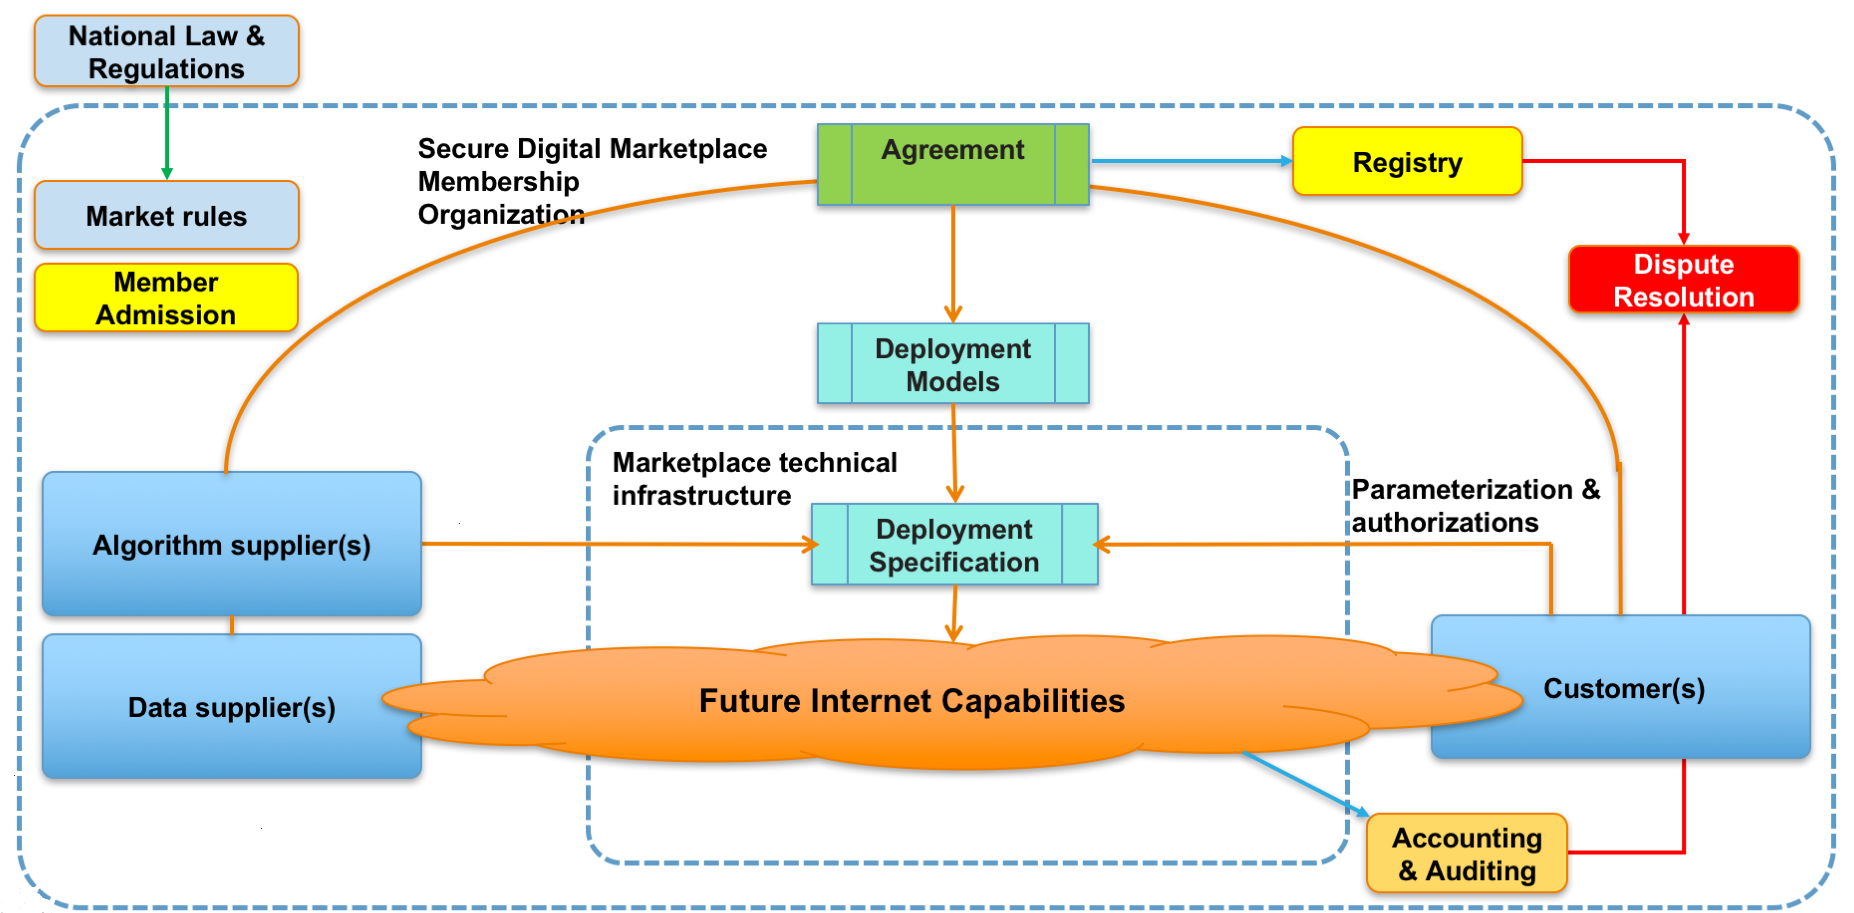
\includegraphics[width=0.9\textwidth]{ch_cmf/market.png}
    \caption{A high-level view of a Data Market Place}
    \label{fig:market}
\end{figure}

Data sharing applications are at the core of operationalization of a DMP. An application defines the flow of processes between collaborating participants, from an organizational standpoint, this translates to defining the duties each participant has to fulfill and restrictions they have to take into account for the application to be performed successfully and in a compliant manner. Once an application is agreed upon by participating actors, there are multiple ways to orchestrate and schedule required actions of the actors. The simplest approach is to create a centralized setting, where there is one center that monitors the actions of the actors and notifies them the next action they have to perform. Although the simplicity of a centralized approach is desirable, it has very strong assumptions. Firstly there is the assumption of observability of all actions where it may not be the case in a real setting. Monitoring a distributed system comes with a cost and this cost is higher if there is one central node that is monitoring all of the system. As opposed to this, distributed and autonomous monitoring, e.g., actors monitoring their local ad-hoc connections is a much more feasible and scalable approach. Secondly it assumes the presence of a fully concretized plan (a series of actions), where in a real setting it may not be the case. Creating fully concrete plans in a setting with many actions and actors is expensive. Furthermore, actors may need to be autonomous with respect to \textit{how} they will perform their part, e.g., delegating parts of tasks or creating local plans based on higher level partial plans in case of failures or to just lower costs while still acting compliant to overall policies. Furthermore, with central planning, the planner node needs to take the all the internal policies of all participants into account to be effective, but in reality the actors may require their policies to remain private resulting planning to be much less feasible.

To solve these issues, the DMP architecture mode proposed in this chapter utilizes a fully distributed control mechanism, where the centralized market actor only defines high-level conditional and context-based duties for actors and provides them with high-level specifications of conditional powers or abilities that they have to perform those duties. Still, the issue of monitoring and accountability remains, having each actor only aware of what it should do will negatively effect trust and cooperation between actors. As it was mentioned in Chapter~\ref{ch:normative_advisors}, apart from letting actors know what they should (and not) do, norms also define expectations that actors can have from others. For a full distributed monitoring setting, the proposed architecture utilizes an ad-hoc monitoring approach, where each actor has expectations, and monitors only the actions in the system that it is also a part of. In summary, between two actors $A$ and $B$, if $A$ has a duty to send a stream of data to $B$, then $B$ is the only actor that is aware of this duty and has an expectation of receiving that data stream. Hence, in effect it is $B$ that is monitoring $A$ and holding it accountable. This chapter argues that distributed governance and control, plus an effective logging and auditing mechanism that can lead to ex-post enforcement can be much more effective in complex cyber-infrastructures than trying to control every aspect of a system with centralized ex-ante access control mechanisms. To demonstrate this approach, next section illustrates an example scenario motivated by~\cite{Zhang2019ModelingPlaces}.

\section{Executable Model of Data Market-Place}
In the scenario, there are four actors, \textit{Alice}, \textit{Bob}, \textit{Charlie}, and \textit{David}. From these actors, \textit{David} needs a set of synthesized data (e.g., a trained model) called \asc{final_result}, to create this data set, first the algorithm \asc{alg1} needs to be executed on a data set \asc{data1} and then the output of \asc{alg1} called \asc{result1} needs to be used as the input of algorithm \asc{alg2} to create \asc{final_result}. The issue is David does not have any of these data or algorithms, instead, Alice has the two algorithms and Bob has the data. The other issue is that Alice and Bob do not trust each other with their data or algorithms (for any reason). However they both trust Charlie whom also happens to have the computational infrastructure. Figure~\ref{fig:dmp-example} a possible solution application that can be utilized in this scenario. The steps of this application are: 
\begin{enumerate}
    \item In any order:
    \begin{enumerate}
        \item Bob sends \asc{data1} to Charlie
        \item Alice sends \asc{alg1} to Charlie
    \end{enumerate}
    \item Charlie executes \asc{alg1} on \asc{data1} to create \asc{result1}
    \item Charlie sends \asc{result1} to Alice
    \item Alice executes \asc{alg2} on \asc{result1} to create \asc{final_result}
    \item Alice sends \asc{final_result} to David
\end{enumerate}


\begin{figure}[t]
\centering
\begin{minipage}[b]{.9\linewidth}
  \centering
  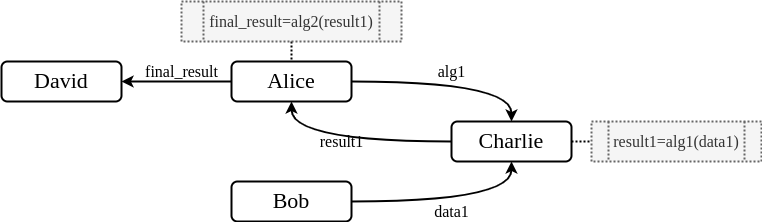
\includegraphics[width=\textwidth]{ch_cmf/market-example.drawio.png}
  \captionof{figure}{DMP Example Scenario}
  \label{fig:dmp-example}
\end{minipage}
\end{figure}

\subsection{Implementation of the Model}
To implement a model of the system, the idea of normative advisors in~Chapter\ref{ch:normative_advisors} is utilized, using ASC2 agents to model the participants of the DMP, and eFLINT to model the contractual agreements of the DMP. 

\subsubsection{Contractual Agreements}
To implement the norms, we first start with a drastically simplified of the general eFLINT specification for concepts in the data-sharing contract presented in Listing~\ref{listing:eflint:dmp-general}. The specification defines two acts \asc{send_data} and \asc{compute} that respectively represent the act of sending a data object (or algorithm) and the act of computing a result based on input data and an algorithm. There are also two duties that correspond to performing the mentioned acts. Note that performance of each act also terminates the corresponding duty. There is also an event defined as \asc{init_contract} that signals the start of a data-sharing contract. Note that the specification is very minimal and generic and not immediately usable, acts do not specify any side effects except terminating the corresponding duties, also the \asc{init_contract} event as it is defined has zero effect on the institutional state. This is because this specification is only there to define concepts and each agent at run-time will get an \textit{specialized} --filled in or concretized-- version of this specification.

% Fact party
% Placeholder source For party
% Placeholder target For party
% Fact data
% Placeholder input For data
% Placeholder algorithm For data
% Placeholder result For data
% Fact reference
\begin{listing}[t]
\centering
\begin{tcolorbox}[left=2pt,right=2pt,top=2pt,bottom=2pt]
\begin{minted}[fontsize=\footnotesize,linenos]{haskell}
Act send_data
  Actor source Recipient target
  Related to data 
  Terminates to_send_data()

Act compute
  Actor source Recipient target
  Related to input, algorithm, reference
  Terminates to_compute()

Duty to_send_data
  Holder source  Claimant target 
  Related to data

Duty to_compute
  Holder source Claimant target
  Related to input, algorithm, reference

Event init_contract
\end{minted}
\end{tcolorbox}
\caption{Generic data-sharing contract notions in eFLINT}
\label{listing:eflint:dmp-general}
\end{listing}

To implement the fully distributed control mechanism, each agent will have its own normative advisor. It is also the goal for each agent to have only access to its own duties and powers, plus the duties and powers of other agents when they are supposed to fully observe them to act as a monitoring point. Building on the specification in Listing~\ref{listing:eflint:dmp-general}, each agent at run-time gets a normative advisor with an specialized \textit{extended} contract specification embedded within it. We start with the simplest specializations, which are David and Bob. Observing the scenario, Bob has only one duty and act to perform --sending \asc{data1} to Charlie -- and no expectations from others while David has no duty or acts to perform while only having one expectation --Alice sending \asc{final_result}-- from other agents. The two Listings~\ref{listing:eflint:dmp-bob} and~\ref{listing:eflint:dmp-david} respectively present the extended specification for Bob and David.


Listing~\ref{listing:eflint:dmp-bob} illustrates Bob's specialized contract. Line 1 instructs eFLINT's reasoners to include the data-sharing basics specification (Listing~\ref{listing:eflint:dmp-general}). Then, line 3 extends the \asc{init_contract} event, so that at the start of the contract Bob has minimal required information about the institutional state of the market-place, i.e., that it has a data set called \asc{data1}, there are two parties Bob and Charlie --from the perspective of Bob-- denoted as \asc{B} and \asc{C}, and that Bob has a power and a duty to send \asc{data1} to Charlie.

\begin{listing}[th]
\centering
\begin{tcolorbox}[left=2pt,right=2pt,top=2pt,bottom=2pt]
\begin{minted}[fontsize=\footnotesize,linenos]{haskell}
#require "data_sharing_basics.eflint".

Extend Event init_contract
  Creates 
    data("data1"),
    send_data("B","C","data1"),
    to_send_data("B","C","data1"),
    party("B"), party("C").
\end{minted}
\end{tcolorbox}
\caption{Bob's data-sharing contract in eFLINT}
\label{listing:eflint:dmp-bob}
\end{listing}



Similar to Bob, David also has a simple extension to its contract specification presented in Listing~\ref{listing:eflint:dmp-david}. It extends contract initialisation event so that it defines two parties Alice and David (\asc{A} and \asc{D}) and also creates a power and a duty for Alice to send \asc{final_result} to David. As the actor/holder of this power/duty is Alice, from the perspective of David it becomes an expectation that David has from Alice, making him a local monitor for this act.

\begin{listing}[h]
\centering
\begin{tcolorbox}[left=2pt,right=2pt,top=2pt,bottom=2pt]
\begin{minted}[fontsize=\footnotesize,linenos]{haskell}
Extend Event init_contract
  Creates  
    send_data("A","D","final_result"),
    to_send_data("A","D","final_result"),
    party("A"), party("D").
\end{minted}
\end{tcolorbox}
\caption{David's data-sharing contract in eFLINT}
\label{listing:eflint:dmp-david}
\end{listing}

Next is Charlie, with the role to get an algorithm and a data set from two other parties, perform the computation and return the results to one of them. An excerpt of Charlie's contract extension is presented in Listing~\ref{listing:eflint:dmp-charlie}. For Charlie, the contract initialization is extended (Line~20) so that it results in creation of two sets of powers/duties: one for Alice to send the algorithm to Charlie and another for Bob to send the data; both of which are expectations from the perspective of Charlie. Then, Charlie's specification also extends the computing act and duty so that they are \textbf{conditionally} created when the initially expected \asc{send_data} are performed (Lines~11 and 15) --more specifically when the \asc{data1} and \asc{alg1} are available--. The compute act is also extended so that when it is performed with the correct parameters, it creates \asc{result1} (Line~7). Finally, the power and duty to send \asc{result1} to Alice is \textbf{conditionally} created when computation is done (Lines~1 and 4) --again, more specifically when \asc{result1} is available--. 

\begin{listing}[h]
\centering
\begin{tcolorbox}[left=2pt,right=2pt,top=2pt,bottom=2pt]
\begin{minted}[fontsize=\footnotesize,linenos]{haskell}
Extend Act send_data
  Holds when source == "C" && target == "A" && data == "result1".

Extend Duty to_send_data
  Holds when source == "C" && target == "A" && data == "result1".

Extend Act compute
  Creates data("result1")
    When input && algorithm && input == "data1" && algorithm == "alg1".

Extend Act compute Holds when source == "C" && target == "A" &&
  input == "data1" && algorithm == "alg1" &&
  reference == "result1".

Extend Duty to_compute
  Holds when source == "C" && target == "A" &&
  input == "data1" && algorithm == "alg1" &&
  reference == "result1".

Extend Event init_contract
  Creates 
    send_data("A","C","alg1"), send_data("B","C","data1"),
    to_send_data("A","C","alg1"), to_send_data("B","C","data1"), 
    party("A"), party("B"), party("C"), 
    reference("result1").
\end{minted}
\end{tcolorbox}
\caption{Charlie's data-sharing contract in eFLINT}
\label{listing:eflint:dmp-charlie}
\end{listing}
%The details on how extensions in eFLINT operate with the \asc{Extend} keyword can be found in~\ref{binsbergen2021b}, but in summary   
Finally, Listing~\ref{listing:eflint:dmp-alice} shows an excerpt of Alice's contract specialization. Contract initialization is extended (Line 13) so a power/duty is created for Alice to send the \asc{alg1} to Charlie. However, this specification also extends the \asc{send_data} act (Line 4) so that when Alice sends \asc{alg1} to Charlie, an expectation for receiving \asc{result1} from Charlie is created. The rest of Alice's specification is similar to Charlie: power/duty to compute \asc{final_result} is created when \asc{result1} is received (omitted Lines 9-11) and power/duty to send \asc{final_result} to David is created when it is available after computation (omitted Lines 1-2). 


\begin{listing}[h]
\centering
\begin{tcolorbox}[left=2pt,right=2pt,top=2pt,bottom=2pt]
\begin{minted}[fontsize=\footnotesize,linenos]{haskell}
Extend Act send_data ...
Extend Duty to_send_data ...

Extend Act send_data
  Creates 
    send_data("C","A","result1"), to_send_data("C","A","result1")
      When source == "A" && target == "C" && data == "alg1".

Extend Act compute ...
Extend Act compute ...
Extend Duty to_compute ...

Extend Event init_contract
  Creates data("alg1"), data("alg2"),
  send_data("A","C","alg1"),to_send_data("A","C","alg1"),
  party("A"), party("C"), party("D"),
  reference("final_result").
\end{minted}
\end{tcolorbox}
\caption{Alice's data-sharing contract in eFLINT}
\label{listing:eflint:dmp-alice}
\end{listing}

\subsubsection{Market Participants}
To fully implement the model of the DMP, after defining the contract specifications for each actor, scripts for intentional agents and normative advisors needs to be created. As an effect of using dynamic norm specifications and normative advisors, we can implement the agent script and normative advisor script in a way that will be usable for all 4 roles. This is immensely important because it means a much higher usability and as a result scalability of development cycle for the models. In short, to define new types of interactions and scenarios, no modification to the agent scripts is required by the modeller. Instead, they can just define new contracts to create scenarios with any number of agents. 


Listing~\ref{listing:advisor:dmp} illustrates parts of the ASC2 script for the DMP advisors agent\footnote{More generic parts that have been already presented in Listing~\ref{listing:advisor} are omitted.}. The two plans that are triggered when a duty \asc{to_send_data} is created or terminated in the embedded eFLINT reasoner. The advisor then simply relays this update to its parent which is a participant agent in the DMP.

\begin{listing}[!tbh]
\begin{minted}[fontsize=\small,linenos]{prolog}
+to_send_data(party(S),party(T),data(D)) =>
    #tell(Parent,send_data(S,T,D)).

-to_send_data(party(S),party(T),data(D)) =>
    #untell(Parent,send_data(S,T,D)).
\end{minted}
\caption{ASC2 specification of DMP participant's norm advisor.}
\label{asc:advisor}
\label{listing:advisor:dmp}
\end{listing}

For a final piece of the model, Listing~\ref{listing:asc2:dmp} illustrates the script for participant agents that act in the DMP. The first plan (Line 1) is for initiation of the contract which simply informs advisor about this event. There are two plans for actual data/algorithm level communications between agents; one for sending a data package (Line 3) and another for receiving a package (Line 7). In both cases the agent also informs the advisor about this. The next three plans are triggered by the advisor: to inform the agent it has a duty to send some data package to a target (Line 10), to inform the agent it should expect to observe a transfer of data, and to inform the agent that a duty to send data has been terminated due to some observed event.

\begin{listing}[!tbh]
\begin{minted}[fontsize=\small,linenos]{prolog}
+!init(Advisor) => !inform_advisor(event,init_contract).

+!send_data(Target,Data) =>
    #tell(Target,package(Data));
    !inform_advisor(act,send_data(Self,Target,Data)).

+package(Data) =>
    !inform_advisor(Act,send_data(Source,Self,Data)).

+send_data(S,T,D) : Self == S =>
    #println("Duty created: " + send_data(S,T,D)).
    !send_data(T,D).

+send_data(S,T,D) =>
    #println("Duty created: " + send_data(S,T,D)).

-send_data(S,T,D) =>
    #println("Duty terminated: " + send_data(S,T,D)).
\end{minted}
\caption{ASC2 specification of a DMP participant}

\label{listing:asc2:dmp}
\end{listing}

\section{Model Execution and Discussion}
Utilizing the illustrated scripts, an executable model of the DMP can be created. This is achieved by the method presented in Chapter~\ref{ch:devops}. For each scenario, a test suite is created with the required type and number of agents. Each market participant agent is created with the script in Listing~\ref{listing:asc2:dmp} and then for each participant a normative advisor is created with the script in Listing~\ref{listing:advisor:dmp} with the corresponding eFLINT specification embedded in it. Then, at the start of the test an \asc{+!init(Advisor)} is sent to each market participant agent where the \asc{Advisor} variable is filled with the name of the corresponding normative advisor agent. Because of the design of ASC2, we can modify different parts of agents by injecting dependencies. With the specific injected communication layer to the agents, we can generate different types of diagrams based on the execution of the system filtered by type of messages, type of agent roles or even just include one specific agent's perspective. In the following, some example insights and artifacts created by execution of the model is presented.



Firstly, Figure~\ref{fig:dmp-seq} illustrates a sequence diagram generated by including only the communications between participant agents (excluding advisors). Intuitively, this generated diagram is a high-level view of the simple scenario contract and can be used as a design artifact for a real system. However as our MAS is scalable to virtually any number of agents, when the system is bigger, this type of artifact generation can be a valuable asset for the designers.

\begin{figure}[!tbh]
\centering
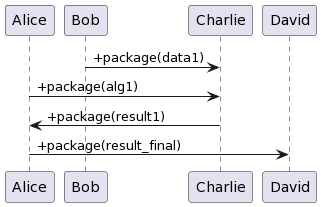
\includegraphics[width=.5\textwidth]{ch_cmf/market-sequence.png}
  \captionof{figure}{Sequence diagram of data-package transfers in the DMP scenario}
  \label{fig:dmp-seq}
\end{figure}

Next, we will focus further on the normative advisors and their interactions with the agents. For this reason, we choose Charlie as the example case. Figure~\ref{fig:dmp-charlie-seq} illustrates a sequence diagram consisting of all of Charlie's communications in the scenario. Charlie initially starts by telling the advisor that the contract started, then the advisor informs Charlie that it should expect two data/algorithm packages from Bob and Alice. When each package arrives, Charlie informs the advisor about it and the advisor tells Charlie that it should no longer expect them, however, after both packages it also informs Charlie that about a new duty towards Alice for a computation. After performing the computation, Charlie informs the advisor about it, and in response, the advisor informs Charlie about the termination of the computation duty and creation of a new duty towards Alice to send the results. After sending the results and informing its advisor, the advisor updates the internal institutional state and informs Charlie about the termination of the duty. As it can be seen, while the external communications of this agent are rather simple, the internal institutional state of the agent is changing rapidly, which in many real world cases is true: even if a behavioral pattern is simple, the underlying interactions that result in those behaviors are complex, in this case the underlying interactions are a legal view over a contractual agreement.

\begin{figure}[!tbh]
\centering
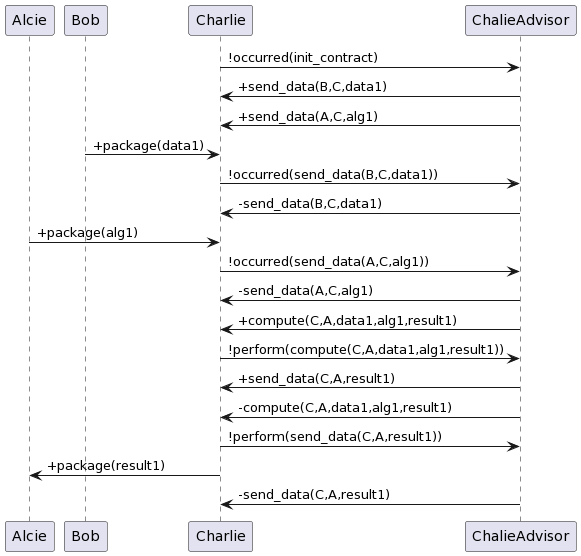
\includegraphics[width=.66\textwidth]{ch_cmf/market-charlie-seq.png}
  \captionof{figure}{Sequence diagram of Charlie's communications the DMP scenario}
  \label{fig:dmp-charlie-seq}
\end{figure}

Finally, we will focus on the concept of local monitoring, deviations between the institutional beliefs of agents and how to identify and possibly synchronize them. The example in Chapter\ref{ch:normative_advisors} presented agents that have identical norms and also identical observations. This meant that the agents had an identical beliefs about the institutional state. However, it the DMP example, this is not the case. While the agents have the same basic concepts in align, each has a specific concretization of norms that it follows. Also, each agent can only observe what is locally available to it: the bilateral communications that it is part of, plus any internal actions that it performs. This has a big effect on accountability in the system, role of trust, need for monitoring and possibility of delegating tasks.

Based on each agent's communications with its advisor, we can create the diagram in Figure~\ref{fig:dmp-example-duties}. This figure shows the discreet life-cycle of duties from the perspective of each agent in the environment. On the bottom there are different events that happen in the system (data packages) which mark the changes in agent's belief about these duties. As it can be seen, these beliefs are not synchronized between agents. For example, David expects to receive the \asc{final_result} from Alice from the moment the contract is initialized. However, Alice has a different view over this and believes this duty only exists when Charlie has sent \asc{result1}. 

   

\begin{figure}[!tbh]
\centering
\begin{minipage}[b]{.9\linewidth}
  \centering
  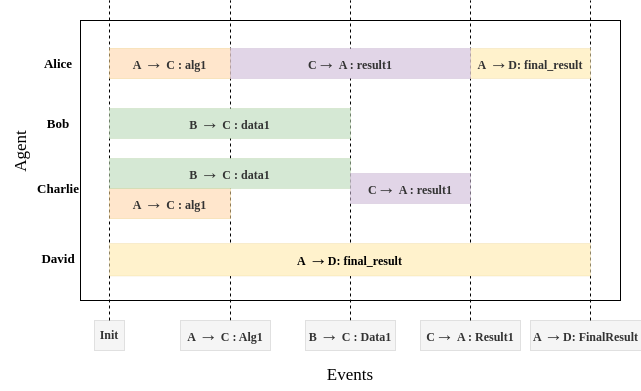
\includegraphics[width=\textwidth]{ch_cmf/duties.drawio.png}
  \captionof{figure}{Discreet life-cycle of duties from the perspective of each agent.}
  \label{fig:dmp-example-duties}
\end{minipage}
\end{figure}

This type of deviation in itself is neither desirable nor undesirable, however, in a complex system it is important that designers are aware of it and can study it. For example, imagine that Bob fails to send the \asc{data1} to Charlie, and then Charlie fails to send the \asc{result1} to Alice, which means Alice can not compute \asc{final_result} for David. Then who should be held accountable from the perspective of David? The answer will depend on the type of agreement between parties. If all of the parties have agreed to be accountable for a task only if previous tasks are completed, then more pre-agreement steps \cite{Baldoni2018} and further monitoring or logging is required in case of failure for possible ex-post auditing and enforcement. But, in case of full delegation, one party may accept to be held accountable for all the sub-tasks that it is delegating to external actors that where not originally part of the agreement --if that is allowed by the policies--. In this case for example, Alice could have an agreement with David to deliver \asc{final_results}, regardless of what happens with other agents, which means there is no need for any further monitoring as David is already (legally) protected by the contract in case of failures.

\section{Conclusion}
This chapter explored a more in-depth analysis of models that can be built by utilizing the tools and frameworks that have been introduced in this thesis. As a proof of concept, a Data Market Place was chosen as the system under scrutiny, and a fully distributed model of task allocation was presented in which the market participants each only get a predefined part a data-sharing agreement specialized for their role that can assist them at run-time to both fulfill their role and coordinate with other participants. To model the participants ASC2 framework was used, also eFLINT was used to model the contractual agreements. Normative advisors as introduced in Chapter~\ref{ch:normative_advisors} were utilized as the glue between the institutional world (contract) and extra-institutional world (data infrastructure).

Although this chapter focused on only modelling the system, in effect, it is not a big leap to implement this approach in a real system in the future: creating and deploying dynamic normative micro-services to advise participants in an ad-hoc or centralized manner and provide them with required information about their and others' roles in a distributed application. Automated norm enforcement and ensuring compliance through explicit and formal representation of norms has many benefits, such approaches can assist both policy-makers and system designers by simplifying their view resulting in a more scalable development process, increase trust between parties and reduce risks that arise from (intended or unintended) non-compliant behaviors. 

While this chapter did not explore the addition of domain, consortium, market, and national policies and legislation, the approach is fully compatible with including external overarching policies. For example, in~\cite{binsbergen2021b} shows how data protection rules (e.g., GDPR) and system level policies can be interconnected. However, this is not a simple matter even from a legal perspective and relations between norms at different levels and their priorities and effects can be much more complex~\cite{hart2012concept}, and they become even more complicated in the context of a cyber-infrastructure that includes large volumes of data, which makes the goals of this thesis, being able to model such interactions much more important.